\documentclass{Project}

\usepackage{graphicx}

\begin{document}
\title{Classifying Primary Emotions in Faces}
\numberofauthors{4}

\author{
\alignauthor Yuxuan Liu \\
       \email{mpanda@live.unc.edu}
\alignauthor Evan Vitkus \\
       \email{vitkuse@live.unc.edu}
\alignauthor Caleb Xu \\
       \email{cjxu@live.unc.edu}
\alignauthor Matthew Zheng \\
       \email{mdz1999@live.unc.edu}
}
\date{7 May 2019}
\maketitle
\begin{abstract}
% Many machine learning applications exist today that are known to be able to identify
% face-like images through the use of facial features. As applications develop, the need for models that are able to identify more than just faces has arisen. One 
% people have been looking into how to extend that 
% feature to determine the more obvious emotion or affect expressed in a picture 
% of a person, such as ``happy", ``sad", or ``angry". \\

% These same processes have varying degrees of success with drawn human 
% characters. By applying the proccesses to drawn human characters, we can
% gauge how accurately models trained on human images are able to analyze and
% draw conclusions from drawn faces, as well as how closely drawn human
% facial emotions approximate their actual human counterparts.
The identification of face-like structures is a problem that had become well-
researched in recent years. While facial-recognition software is becoming more and more
accurate, the messages and implications contained in the emotions of the person 
are often lost when still images are captured. Additionally, this software is often
lackluster when used on cartoon faces. In this paper, we create various 
models to attempt to analyze images, both real and cartoon, to identify the emotions
portrayed in the faces based on a set of facial landmarks with models trained on 
real facial data reaching 62\% and models trained on cartoon faces reach 98\% accuracy.
We were able to conclude that the way that emotions are portrayed in real faces 
are relatively consistent with other real faces and similar for cartoon faces. 
However, cartoon and real faces have little in common with their landmarks differing 
significantly with accuracy levels around 25\%. 

\end{abstract}

\section{Introduction}
As machine learning models have been on the forefront of research in nearly every 
field of study, the use cases and applications of such models has rapidly broadened. 
With the models able to form accurate predictions given pre-existing data, the use
of such models is immensely attractive in fields that present difficult problems that
have large amounts of existing data. One particular field of study that has attracted
much interest in recent years is the identification of emotions. Understanding the 
emotions that a person is experiencing is critical in understanding the meaning and 
intention behind their disposition; however, as a naturally subjective trait,
emotions are often misunderstood resulting in confusion and uncomfortable situations.
While possible to detect a person's emotions based on their actions, this is often 
still subjective and is often too late. 

Emotions are displayed through a variety of means known as affect displays. These
affect displays are sometimes sufficient to determine emotion, but are not always
comprehensive. Additionally, even if an emotion is perceived it is often difficult 
to understand why that perception occurs. While it may be obvious to say a person 
is expressing the emotion of joy when they are smiling, it doesn't capture every 
feature that the brain takes into account in processing the expression. In 
a different facial context, a smile could also indicate another emotion 
such as awkwardness or surprise.\\

With the subjective nature of emotions and the inability to properly identify the 
meaning of particular affect displays without additional information, it can be
difficult to identify emotions that are artificially displayed. For example, when drawing,
digital artists must render emotions as they believe they would appear. Then, the 
consumer will interpret the digitally produced face. This can result in an image 
that displays emotion incorrectly or in a manner that is difficult to perceive. 
As a result, messages can be warped or misinterpreted. It is therefore imperative 
that we create models capable of quantitatively interpreting emotions.

Current research has shown that an effective way of determining emotion is through 
the Facial Action Coding System (FACS). \cite{tian_kanade_cohn_2001}
This system makes use of action units, particular facial movements such as the 
raising of cheeks of the dropping of the jaw to identify the emotion expressed 
on a face. With animated or cartoon faces, however,
these action units can not be relied on. These faces often lack certain of these
action units and would therefore be unidentifiable with FACS. 

Since we can not rely on FACS due to the lack of captured motion, we decided to
analyze the known 68 facial landmarks. Using these landmarks, we can understand
the position of pieces of the face that encompass the action units. Using 68 
landmarks we seek to train models capable of identifying the emotions present
in images of faces both real and cartoon. We then cross-test these models to see
how closely real and cartoon faces' landmarks are to one another. Finally, we
train a model on a combination of the data. Using these models, we seek to determine 
how closely related real and cartoon faces are, and how accurately emotions are 
displayed in them.

\section{Approach}
In order to detect emotions through facial expressions, we required many 
images of faces and a way to quantify their expressions. We acquired two datasets, the 
Facial Expression Research Group Database (FERG-DB) from Washington University
and Karolinska Directed Emotional Faces (KDEF) from the Emotion Lab at the Karolinska Institutet.
\cite{aneja2016modeling}\cite{KDEF}  
The FERG-DB dataset is a collection of six cartoon people displaying
a variety of emotions and the KDEF dataset is of 140 real people displaying the 
same set of emotions taken from a variety of angles. Both of these datasets' images
had been previously classified with emotions. To quantify the facial landmarks
in these, we created a histogram of oriented gradients (HOG).\cite{geitgey_2016}
With our newly fashioned, quantified dataset we ran multiple classifier machine
learning algorithms to produce sets of models to determine the accuracy of the
emotions expressed. Using scikit-learn, we created five separate model sets
where we trained and tested on cartoon to cartoon, real to real, cartoon to
real, real to cartoon, and a combination of cartoon and real to a 
combination of cartoon and real respectively. \cite{scikit-learn}

\begin{figure}[h!]
  \centering
  \begin{minipage}[b]{0.4\linewidth}
    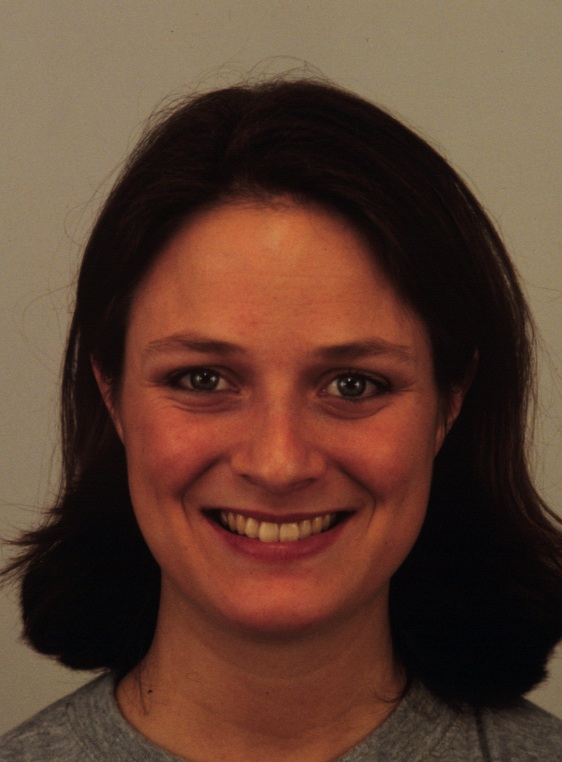
\includegraphics[width=\linewidth]{AF01HAS.JPG}
  \end{minipage}
  \begin{minipage}[b]{0.4\linewidth}
    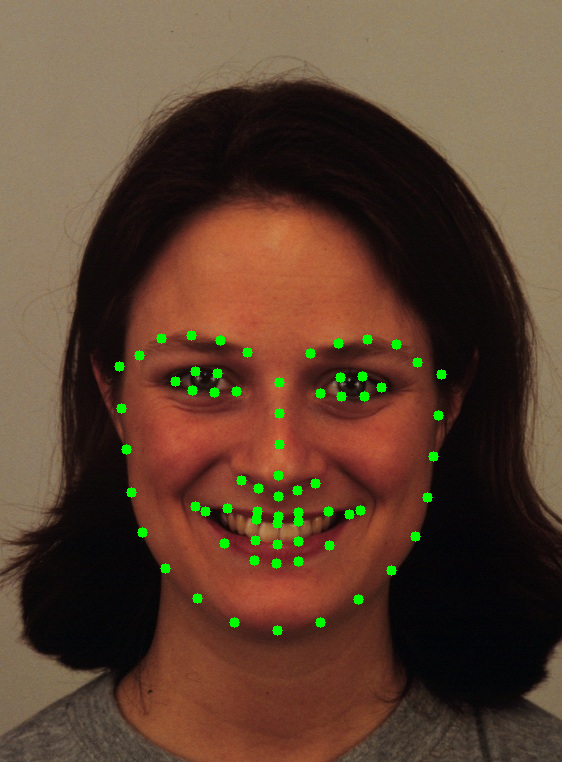
\includegraphics[width=\linewidth]{AF01HAS_annotated.png}
  \end{minipage}
  \caption{Comparison of original face with marked face from KDEF dataset}
  \label{fig:happyReal1}
\end{figure}

\begin{figure}[h!]
  \centering
  \begin{minipage}[b]{0.4\linewidth}
    
\includegraphics[width=\linewidth]{aia_anger_127.png}
  \end{minipage}
  \begin{minipage}[b]{0.4\linewidth}
    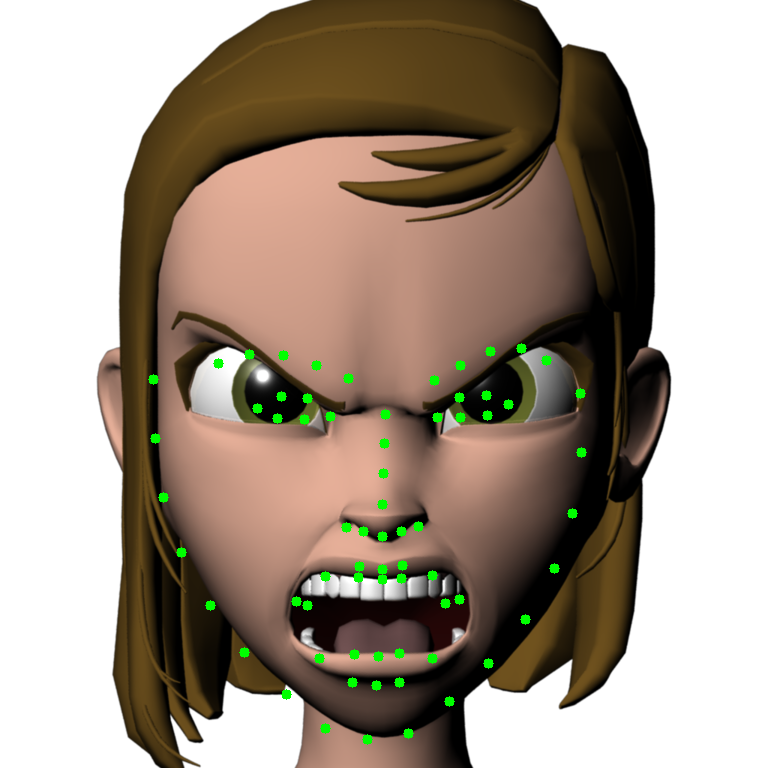
\includegraphics[width=\linewidth]{aia_anger_127_annotated.png}
  \end{minipage}
  \caption{Comparison of original and marked face from FERG-DB dataset}
  \label{fig:happyReal1}
\end{figure}

\section{Procedure}
After obtaining image data from FERG-DB and KDEF datasets, we ensured that all
of the images were the same size. The KDEF images feature subjects from frontal
and side camera angles. To ensure consistency with angles of images used from
the FERG-DB dataset, we filtered the KDEF images to use only images captured
from a direct frontal angle. \\

The FERG-DB images were already at the resolution of $768 \times 768$, 
while the KDEF images were at the resolution of $562 \times 762$.
To address this discrepancy, all of the images were padded
with plain white on left and right to the resolution $762 \times 762$ before
being rescaled to resolution $768 \times 768$ through bicubic resampling in
order to match the FERG-DB image sizes. These image resizing operations are
implemented in \texttt{image\char`_resize.py}. \\

Using pre-trained model files for \texttt{dlib}, we then generated 68 landmark
coordinates for each FERG-DB and KDEF image.\cite{dlib-models}\cite{dlib09}
These landmark generation operations are implemented in 
\texttt{cartoon\char`_bulk\char`_face\char`_detector.py}
and \texttt{real\char`_bulk\char`_\\*face\char`_detector.py}, respectively. \\

These landmarks are stored in \texttt{real\char`_landmarks.csv}
and \texttt{cartoon\char`_landmarks.csv}. The emotion labels for these images
were also quantized from one to seven, corresponding to anger, disgust, fear,
joy, neutral expression, sadness, and surprise, respectively, and these labels
are then stored in \texttt{real\char`_labels.csv}
and \texttt{cartoon\char`_labels.csv}. The order of entries in each landmarks
file corresponds to that of the entries in the respective labels file. \\

These landmark and label sets are then processed in
\texttt{csv\char`_pro\-cess.sh}. The cartoon and real landmarks and labels are
shuffled, and then a new landmark and label file containing equal parts of
cartoon and real data is generated. The cartoon and real landmarks and labels
are then also divided by a 75-25 split into training and test data,
respectively. Finally, we train machine learning models in
\texttt{sklearn-templ\-ate.py}. The script takes two arguments, each being one of
the words \texttt{real}, \texttt{cartoon}, or \texttt{combined}. The first
argument selects the dataset upon which to train the models, and the second
argument selects the dataset upon which to test the models. For example, the
invocation \texttt{python sklearn-template.py cartoon real} will train the
models on the cartoon face dataset and test them on the real face dataset.
Without any arguments, the script will train and test all possible combinations
of real, cartoon, and combined datasets. \\

The Python script produces an output file, \texttt{sklearn\char`_outpu\-t.csv},
showing the percentage of accuracy of each of the models trained and tested in each
combination. The script trains a number of models in \texttt{sklearn},
including a random forest ensemble classifier, Ada Boost classifier, bagging
classifier, extra trees classifier, gradient boosting classifier, and decision
tree classifier.

\section{Results}

As seen in Table 1, our model performed stronger on the cartoon faces than the real faces for every model we ran. Comparing each model's performance, each model predicted emotion more accurately on the cartoon image than on the real face. Our justification is due to the variance among faces. Our cartoon data was a compilation of six individuals, each with over 9,000 images. The KDEF dataset involved 140 different participants with only 8 viable images each. Our strongest performing model was gradient boosting followed by random forest. We received the most accurate models when comparing among the same data. This follows because there is less variance when predicting among the same dataset. We also received a lower average prediction score from our combined datasets. The reason also has to do with additional variance between the real and cartoon faces. The combined model performs better than trying to directly cross-compare because we are training on the both datasets.
\begin{table}[h!]
\centering
\caption{\textit{Training results on datasets within themselves}}
\begin{tabular}{|c|c|c|} \hline
\textbf{Model}      & \textbf{Real $\rightarrow$ Real}  & \textbf{Cartoon $\rightarrow$ Cartoon}  \\\hline
Random Forest       & 0.567346                          & 0.981730  \\\hline
Ada Boost           & 0.432653                          & 0.617876  \\\hline
Gradient Boosting   & 0.624489                          & 0.956037  \\\hline
Decision Tree       & 0.424489                          & 0.898318  \\\hline
\end{tabular}
\end{table}

\begin{table}[h!]
\centering
\caption{\textit{Training results on datasets between each other}}
\begin{tabular}{|c|c|c|} \hline
\textbf{Model}      & \textbf{Real $\rightarrow$ Cartoon} & \textbf{Cartoon $\rightarrow$ Real}  \\\hline
Random Forest       & 0.276512                            & 0.208163  \\\hline
Ada Boost           & 0.262755                            & 0.297959  \\\hline
Gradient Boosting   & 0.292452                            & 0.277551  \\\hline
Decision Tree       & 0.230438                            & 0.228571  \\\hline
\end{tabular}
\end{table}

\begin{table}[h!]
\centering
\caption{\textit{Training results on combined dataset within itself}}
\begin{tabular}{|c|c|c|} \hline
\textbf{Model}      & \textbf{Combined $\rightarrow$ Combined} \\\hline
Random Forest       & 0.542857  \\\hline
Ada Boost           & 0.318367  \\\hline
Gradient Boosting   & 0.585714  \\\hline
Decision Tree       & 0.402040  \\\hline
\end{tabular}
\end{table}

\section{Conclusions}
With the accuracy that we've obtained from the different models, we've 
established several things. To no surprise, real faces and cartoon faces proved
to be solid datasets to use to classify themselves. Real to real achieved 
upwards of 62\% accuracy while cartoon to cartoon achieved upwards of 98\% 
accuracy in classification with certain models. While real to real produces a 
weaker classifier, we believe that is due to the small size of our real face dataset.

The part that is interesting is that classifying one type using the other type 
as a training set is not very accurate. Most models using one set to classify the
other barely does better than random guessing. Even trying to combine the training sets produced lackluster, 
although better, accuracy. The improved accuracy, however, can be attributed to the large size of the FERG-DB 
data set allowing for a large number of cartoon faces to be classified correctly.

One possible explanation for the inefficacy of the cross-tested models could be that we simply didn't have 
enough data in the KDEF data set. This explanation doesn't hold up well, however, because we had a decently 
large training set when using the cartoon set to train but it still produced an inaccurate classification for 
real datasets. 

Another possible explanation is the radical difference between the two datasets. As a result, the model might 
as well be guessing as the landmarks on cartoon faces potentially do not match up or align at all with their 
real counterparts. In fact, visual inspection shows that the landmark features on the cartoon faces are often 
exaggerated compared to their realistic counterpart.

We may be tempted to conclude that there actually exists some amount of correlation between the landmarks on 
the real faces and on the cartoon faces. However, the accuracy of the cross-tested models is not significant 
enough to account for the randomization of the classification that inherently existed in the datasets.
Since people are inherently imperfect at identifying and/or creating human facial expressions, it is unsafe to 
assume that the results are significant. The evidence only supports the claim that cartoon faces bear little 
resemblance to their real counterparts. 

\section{Future Work}
Possible follow up to improve our models would be increasing the number of facial landmarks and a general 
increase in the size of the real face image data set. A larger dataset for real faces would grant our model 
additional data to train with, resulting in better classification power. Additionally, with a larger number of 
facial landmarks per image, additional information about each image would be added as quantifiable information.
More landmarks would result in a better depiction of the face by providing our data with additional contours to
each face. \\

Another interesting way to interpret these findings would be to create or find a dataset where each real face
has a cartoon face counterpart that is produced to be a replica of the real face. This will not only produce a
more accurate model but will also better answer the question of whether people could intentionally produce
artificial emotions in cartoons.

Additional interesting directions to continue with our research include adding images of faces in a natural
environment, which includes having faces that are not oriented directly towards the camera and the generation
of more natural cartoon faces displaying particular emotions. 

%
%You can also use a citation as a noun in a sentence, as
% is done here, and in the \citeN{herlihy:methodology} article;
% use \texttt{{\char'134}citeN} in this case.  You can
% even say, ``As was shown in \citeyearNP{bowman:reasoning}. . .''
% or ``. . . which agrees with \citeANP{braams:babel}...'',
% where the text shows only the year or only the author
% component of the citation; use \texttt{{\char'134}citeyearNP}
% or \texttt{{\char'134}citeANP}, respectively,
% for these.  Most of the various citation commands may
% reference more than one work \cite{herlihy:methodology,bowman:reasoning}.
% A complete list of all citation commands available is
% given in the \textit{Author's Guide}.

%\end{document}  % This is where a 'short' article might terminate

%ACKNOWLEDGEMENTS are optional
\section{Acknowledgements and Citations}
We would like to acknowledge Jorge Silva for instructing us in COMP 562 and providing
with the starting ground for this research. We also thank Washington University and 
the Karolinska Institutet for allowing us to use their data.

% The following two commands are all you need in the
% initial runs of your .tex file to
% produce the bibliography for the citations in your paper.
\bibliographystyle{abbrv}
\bibliography{bibfile}  % sigproc.bib is the name of theBibliography in this case
% You must have a proper ".bib" file
%  and remember to run:
% latex bibtex latex latex
% to resolve all references
%
% ACM needs 'a single self-contained file'!
%
%APPENDICES are optional
% SIGKDD: balancing columns messes up the footers: Sunita Sarawagi, Jan 2000.

% That's all folks!
\end{document}
